\title{\textrm{deSQLifier (5)}}
\author{
        Kia Rahmani \\
                Department of Computer Science\\
        Purdue University, USA
}
\date{\today}
% Main Document
\documentclass[12pt,letter]{article}
\usepackage{xcolor,listings}
\usepackage{graphicx}
\usepackage{wrapfig}
\usepackage[inline]{enumitem}
\usepackage[utf8]{inputenc}
\usepackage[english,ngerman]{babel}
\usepackage{csquotes}

\begin{document}
\selectlanguage{english}
% \maketitle
%\begin{abstract} \end{abstract}

% ---------------------------------------------------
% ---------------------------------------------------
% Sections ------------------------------------------
% ---------------------------------------------------
% ---------------------------------------------------
\section{Evaluation}
In this section, we will present results from our empirical studies and
experiments showing the practicality of eventual consistency (ES) as a
notion of
correctness for  applications
derived from two main sources. Additionally, we will show how naive
enforcement
of ES (or any other notion of correctness) will result in loss of either
performance or correctness and we will
consequently present our provably correct and optimized 
database isolation requirements for a corpus of real-world and theoretical
applications.


\subsection{Benchmark and real-world applications}
\begin{center}
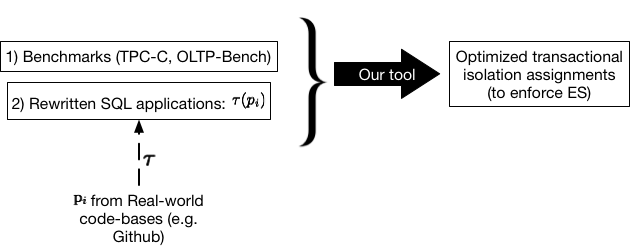
\includegraphics[scale=0.45]{figures/outline.png}
\end{center}
The above figure shows the outline of our analysis. In order to show usability
of our tool, we performed an extensive study of SQL programs, including (but not
limited to) eCommerce, banking, warehouse management, all derived from either of
the following two sources: 
\paragraph{i) Benchmark applications:} 
We gathered a large set (about 10) of benchmark applications that are all
widely used for
industrial or academic prototype benchmarking. Detailed descriptions of
these
applications are publicly available and there is a consensus in the
database
community on their \emph{correct behavior} (in some cases, e.g. TPC-C, the
applications
level invariants are explicitly specified).

\paragraph{ii) Real-world applications:} 
In addition to the above benchmarks, we also
gathered a corpus of popular Ruby-on-Rails applications from Github and
analyzed them using our tool. Since our general-purpose analysis tool
targets
generic database-backed applications as opposed to any specific development
framework, we had to transfer the Rails applications into simpSQL. In order
to
facilitate this process, we created a (to be precise, expanded an already
existing)
tool to execute Rails applications symbolically and create an equal simpSQL
program which then we were able to analyze using our tool. The
transformation is
shown by $\tau$ in the above figure and is fairly straightforward (although
we
do not present any formal proof of equivalence for $p$ and $\tau(p)$).

\subsection{Evaluation of ES as a notion of correctness}
In this section, we will present emprical evidence supporting our choice of ES
as the right notion of application correctness. 

\begin{wrapfigure}{r}{0.1\textwidth}
  \begin{center}
    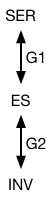
\includegraphics[scale=0.5]{figures/gaps.png}
  \end{center}
\end{wrapfigure}
Specifically, we will first show that,
ES preserves \emph{all (high-level) invariants} that programmers need (i.e. it
is not too weak in practice). 
Second, we will  show that ES is not too strong; that is: 
\begin{enumerate}
  \item G1 gap is not too small, i.e. there is a considerable number of cases where SER is violated 
        but ES is not. 
  \item G2 gap is not unnecessarily big, i.e. we inspect all cases where ES is
    violated but invariants are not, and we argue that there are in fact
    other (arguably important) invariants that are being violated and thus
    ES is actually helping developers who might forget to specify all of
    their requirements.
\end{enumerate}

In the following sections, we will consider two classes of invariants: \emph{explicit
invariants} (e.g. associations and validations on Rails Active Records) and
\emph{implicit invariants}, which are widely discussed and accepted in the
literature as requirements for applications (e.g. non-negative inventories
and account balances for many eCommerce applications \cite{Bailis:Feral}).


\subsubsection{correctness}
Here we will show that ES can be safely used as the notion of
correctness for all examined applications. Specifically, we need to show
something like the following arguments (the degree of formal rigorousness is debatable for a SIGMOD
submission):
\begin{enumerate}
  \item Given a Rails program $p_r$ and the conjunction of its invariants
    $INV_r$, the transformation $\tau$ returns \emph{equivalent} SQL
    program and invariants, $(p_s,INV_s)$. That is, for any given history $H_r$ of $p_r$ that preserve
    $INV_r$, 
    there exists a history $H_s$ that is \emph{observably} equal to $H_r$
    and preserves $INV_s$.

  \item Then we need to show that in all the studied applciations, all SQL histories that preserve $ES$ also presereve $INV_s$.
\end{enumerate}

\subsubsection{efficiency}
Here we will show how often SER is violated in real-world applications but
ES is not. We applied our tool twice on each application (once looking for
SER violations and once modified for ES violations) and the following
results show that in x\% of the transactions are ES-safe under default
isolation level of the deployed database but are not SER-safe.
(or in another approach, we can show that x\% of the transactions are
assigned a weaker isolation guarantee when ES is enforced as opposed to
SER).

Additionally, by analyzing ES anomalies found by our tool, we report in
almost all of them some invariant (explicit or implicit) also being
violated. In the rare cases where no invariant is violated, we found
critical problems on some objects (objects not specified by the developer
in any invariant for example) which we argue that are able to break the
whole functionality of the program.

%%%%%%%%%%%%%%%%%%%%%%%%%%%%%
\subsection{Correctness Enforcement}
In this section, we present empirical results on the performance gained by
our optimal ES enforcement approach. Our results show y\% performance gain
over a naive (or default) enforcement technique, where all database
transactions are
serializable (default). Our tool additionally offers a bounded correctness
guarantee, which the following experiment results (with a number of
concurrent
transactions much higher than the bound) support the claim that is
enough to find and fix real-world problematic applications
(for example, we can run TPC-C on the default transactions of the database
and show
invariants are violated, and then by applying our tool and finding the
necessary isolation levels, we can run it again with thousands of
concurrent clients and show no invariant is violated).

As an additional result, we also show the performance gain from replacing
ES with SER as the enforced correctness criteria in a real-world setting.
\subsection{Comparison to related works}
\paragraph{ACIDRain: Concurrency-Related Attacks on Database-Backed Web
Applications\cite{Bailis:Acid}:}
We share the goal of finding the possibility of anomalous application
behaviors
on weakly isolated transactions with this paper. However, instead of a
simple syntactic
analysis, we offer a fully automated tool which captures the semantics of
the
programs and reports less false alarms (with the addition of the bounded
guarantee). For example, in the paper they mention:
\begin{displayquote}
``... the second class of false positives were due to anomalies that were in fact
triggerable but were handled by other program logic and thus rendered
benign.''
\end{displayquote}
Here, we will present our reults showing how our tool is able to detect
cases like above and report actual errors more accurately. 


\paragraph{Serializability for Eventual Consistency: Criterion, Analysis, and
Applications\cite{Vechev:Ser}:} Unlike this paper, we target ES (instead of
SER) as the
correctness notion which liberates us from manual interactions with the
tool such as the folllwings: 

\begin{displayquote}
``... For the sake of the experiment, we exclude from our analysis queries issued
within declared rendering sections of TOUCHDEVELOP scripts, as they are
very frequently executed (every time a page is re-rendered), guaranteed to
have no side effects on the program state, and are almost always harmless
in practice.''
\end{displayquote}
or 
\begin{displayquote}
``...  Therefore, we chose performance over strong consistency in this case by
  adding a lightweight annotation to exclude the queries in the above
  figure from the serializability checking. With similar reasoning, we can
  resolve several other violations.''
\end{displayquote}

\paragraph{Feral Concurrency Control:
An Empirical Investigation of Modern Application
Integrity\cite{Bailis:Feral}:} 
Similar to \cite{Bailis:Acid}, here also they perform a simple syntactic
analysis on the programs and thus are prone to false errors. In addition,
their tool is specifically designed for Rails applications while ours is
supporting a generic SQL language which can be used for all database backed
applications. Finally, we do not consider high-level invariants as the
notion of correctness, which as we have already shown can be problematic in
practice. 

\paragraph{Alone Together: Compositional Reasoning and Inference for Weak
Isolation\cite{Kaki:Alone}:}
They do not offer any evidence of the applicability of their tool in
practice, while we have extensive study results using our fully automated
tool (maybe we need a
better argument here...)







% The Biblography
\bibliographystyle{abbrv}
\bibliography{../kia-bib}
\end{document}
